\documentclass[00-livre-main.tex]{subfiles}
\begin{document}

\chapter{The Equation of a Line in the Plane}


Let's recall the idea of \emph{the plane} from classical geometry: the plane is like a flat sheet of drawing paper, which extends indefinitely in all directions without bound. 
It is the playground for lots of serious considerations from high school: points, lines, circles, triangles, rectangles, and various other doodles live in it. 
I say \emph{in} it rather than \emph{on} it, because all of those objects really have their existence inside the plane. 
If we were to say ``on the plane'' then one might think of them as sitting on top of the paper, where a light breeze might move them about. 
No, those things live inside the plane just as sure as you and I live inside the universe.

And while all of that is evocative and romantic, it doesn't make doing mathematics any easier. 
Our aim in this first chapter is to do some concrete mathematics: we want to figure out how to describe a single line in the plane very carefully. 
To do this, we will use tools that Ren\'{e} Descartes taught us: coordinates. 
Better yet, we will use an update of the idea and introduce \emph{vectors}. 
Our work has to rely on something, so at some points we will make use of geometry facts you learned in high school. 
But for all of the points and vectors, angles and dot products, we will go straight to the heart of a single important question:

\begin{quotation}
\textbf{\large How can we clearly describe a single line in the plane with an equation?}
\end{quotation}

\clearpage

\section*{Points, Vectors, and Vectors}


You have likely seen the idea of \emph{Cartesian coordinates} on the plane before. To be clear, let's set things down carefully. In the plane, we choose a pair of perpendicular lines which meet at a point $O$. This special point is called the \emph{origin}. Then, we choose a point $X$ on one of the lines and draw the circle centered at $O$ which passes through $X$. Note that this circle meets our two lines in two points each, four points total, one of which is the point $X$. Then, from $X$, we rotate around the circle by a quarter turn counterclockwise until we hit one of the points on the other line. This new point we will call $Y$. Are you drawing with me? Here is my picture so far.

\begin{figure}[h!]
\centering
\begin{tikzpicture}[scale=2]
\draw (-1,4/3) -- (1,-4/3);
\draw (-3/2,-9/8) -- (3/2,9/8);
\draw (0,0) circle [radius=3/4];
\draw[->] (-50:1) arc (-50:35:1);
\node [right] at (1.1,0) {rotate counterclockwise};
\node [left] at (0,0) {$O$};
\node [below] at (9/20,-3/5) {$X$};
\node [above] at (3/5,9/20) {$Y$};
\end{tikzpicture}
\end{figure}

We call the line $OX$ the \emph{$x$-axis} and the line containing $Y$ the \emph{$y$-axis}. Here comes the amazing part: we declare the circle we used to be of \emph{unit size}, and make the lines $OX$ and $OY$ into number lines! The important part is that the point $O$ should represent $0$ on both number lines, and the points $X$ and $Y$ should each represent $1$ on their lines. So, instead of marking things with $O$, $X$, and $Y$, we put down marks where $X$ and $Y$ are and label them with $1$'s, and add little arrows marked with $x$ and $y$ near the positive ``ends'' of the lines $OX$ and $OY$, respectively.

\begin{figure}[h!]
\centering
\begin{tikzpicture}[scale=1.25]
\draw[->] (-1,4/3) -- (1,-4/3);
\draw[->] (-3/2,-9/8) -- (3/2,9/8);
\draw[fill] (9/20,-3/5) circle [radius=0.03];
\draw[fill] (3/5,9/20) circle [radius=0.03];
\node [below] at (9/20,-3/5) {$1$};
\node [above] at (3/5,9/20) {$1$};
\node [right] at (1,-4/3) {\small $x$};
\node [left] at (3/2,9/8) {\small $y$};
\end{tikzpicture}
\end{figure}

Note that above I have done something a bit silly and let the picture just fall on the paper in an unusual way. 
I really mean unusual as ``not usual.'' 
The usual way arranges the lines on the paper to match our expected horizontal ($x$) and vertical ($y$) directions. 
This isn't actually required, but it is what everyone always does. 
So, the more typical picture looks more like this one.


\begin{figure}[h]
\centering
\begin{tikzpicture}[scale=1.25]
\draw[->] (-2,0) -- (2,0) node[below] {\small $x$};
\draw[->] (0,-2) -- (0,2) node[left] {\small $y$};
\draw[fill] (1,0) circle [radius=0.03] node[below] {$1$};
\draw[fill] (0,1) circle [radius=0.03] node[left] {$1$};
\end{tikzpicture}
\caption{The Standard Cartesian Coordinate System}
\end{figure}


Now suppose we have some point in the plane, let's call it $P$. 
We can describe the location of $P$ relative to our two lines in a simple way. First, we draw a line through $P$ which is parallel to the $y$-axis and perpendicular to the $x$-axis.
The foot of this perpendicular hits the $x$-axis at some point $A$.
But this point $A$ is part of the number line $OX$, so it has an associated real number, which we will call $a$.
So the point $A$ is instead marked with the label $a$ from this number line.

Similarly, we draw a line through $P$ parallel to the $x$-axis and perpendicular to the $y$-axis.
The foot of this perpendicular hits the $y$-axis at some point $B$, which is part of the number line $OY$.
We denote the number associated to $B$ by $b$. 
Again, the point is labeled with the number $b$ from the number line.

\begin{figure}[h!]
\centering
\begin{tikzpicture}[scale=1.2]
\draw[->] (-2,0) -- (2,0) node[below] {\small $x$};
\draw[->] (0,-2) -- (0,2) node[left] {\small $y$};
\draw[fill] (-1/2,3/4) circle [radius=0.03] node[below left] {$P$};
\draw[dotted] (-1/2,-2) -- (-1/2,2);
\draw[dotted] (-2,3/4) -- (2,3/4);
\draw (-.05,3/4) -- (.05,3/4) node[above right] {$b$};
\draw (-1/2,.05) -- (-1/2,-.05) node[below left] {$a$};
\end{tikzpicture}
\caption{A point $P$ and its coordinates $(a,b)$.}
\label{fig:point-coords}
\end{figure}

So, to identify the point $P$, we can instead give the pair of numbers $a$ and $b$. 
These numbers are called the \emph{coordinates} of $P$.
Of course, the order of the coordinates matters, so we make what we call an \emph{ordered pair} $(a,b)$ to keep things straight, where the $x$-coordinate comes first, and the $y$-coordinate comes second. Note that in Figure \ref{fig:point-coords} the $x$-coordinate $a$ is negative, but the $y$-coordinate $b$ is postive.

This whole process is reversible, too. If we pick a pair of numbers $c$ and $d$, in order, then we can find a point in the plane which corresponds, and we can do it unambiguously. Find the spot labeled $c$ on the $x$-axis number line and construct a line perpendicular to the $x$-axis through this point. Similarly, find the spot labeled $d$ on the $y$-axis and construct a line perpendicular to the $y$-axis through this point. The two lines you just drew will meet in exactly one point $Q$, and $Q$ will have coordinates $(c,d)$.

\vspace{.5cm}
\hrule
\vspace{.5cm}

This setup of coordinates on the plane allows us to formalize a wonderful and useful idea from physics, too. 
Physicists use the concept of a \emph{vector} to describe something (like the wind) which has both magnitude or size (like how fast the air is moving)  and direction (which way the air is going).
Usually, vectors are drawn as little arrows: the arrow has a direction, and it has a length which represents its magnitude.
It is possible to draw vectors which have the same direction but different lengths, and vice versa.

We can use coordinates to describe vectors in the plane, too. 
Here's how: A physicist's vector $V$ is some arrow in the plane.
That arrow has an initial point $P$ and a final point $Q$.
We can write the coordinates of these points as $P = (a,b)$ and $Q = (c,d)$.

\begin{figure}[h]
\centering
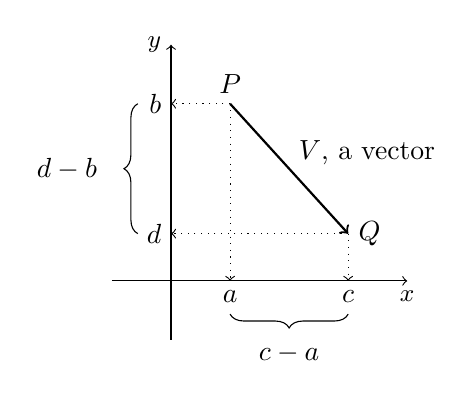
\begin{tikzpicture}[scale=1.5]
\draw[->] (-.5,0) -- (2,0) node[below] {\small $x$};
\draw[->] (0,-.5) -- (0,2) node[left] {\small $y$};
\draw[->,thick] (1/2,3/2) node[above] {$P$} -- (3/2,2/5) node[right] {$Q$};
\node [above right] at (1,18/20) {$V$, a vector};
\draw[dotted,->] (1/2,3/2) -- (1/2,0) node[below] {$a$};
\draw[dotted,->] (1/2,3/2) -- (0,3/2) node[left] {$b$};
\draw[dotted,->] (3/2,2/5) -- (3/2,0) node[below] {$c$};
\draw[dotted,->] (3/2,2/5) -- (0,2/5) node[left] {$d$};
\draw[decorate,decoration={brace,amplitude=5pt},xshift=-8pt,yshift=0pt] (0,2/5) -- (0,3/2) node[midway,xshift=-.9cm] {$d-b$};
\draw[decorate,decoration={brace,mirror,amplitude=5pt},xshift=0pt,yshift=-8pt] (1/2,0) -- (3/2,0) node[midway,yshift=-.5cm] {$c-a$};
\end{tikzpicture}
\caption{Coordinates for a physicist's vector $V$.}
\label{fig:phys-vec-coords}
\end{figure}


Then the coordinates of $V$ are taken to be the numbers $c-a$ and  $d-b$, which we interpret how much $V$ acts in the directions parallel to the $x$-axis and the $y$-axis, respectively. 
Note that in Figure \ref{fig:phys-vec-coords}, the $y$-coordinate is negative, since $b>d$.

These coordinates have a hint of algebraic manipulation in them. 
Those subtractions line up almost like we could write $V =(c-a,d-b) = (c,d)-(a,b) = Q-P$. 
But $V$ is a vector, and if we write it like $(c-a,d-b)$, it looks like the notation for a point. 
We should not do that because it could get confusing.
Furthermore, that ``equation'' would mean that we are subtracting points and creating a vector, which is also weird.
Still, there is something there.
We will return to this idea soon.

For now, let's focus on a bit of ambiguity in the physicist's idea of a vector. 
Where should that vector be?
That is, given the coordinates of a vector in the plane, it is not clear where to draw it!
I can slide a vector around the plane, and as long as I keep it parallel to the original, the coordinates won't change. 
So, unlike with the coordinates of a point, the coordinates of a vector do not uniquely specify the vector.

The mathematician's special fix is this: we simply declare all our vectors to have their initial points, their tails, at the origin $O$, of our coordinate system.
That curtails some of the (admittedly useful) freedom in the physics notion, but it also lets us be more clear.

\begin{figure}[h]
\centering
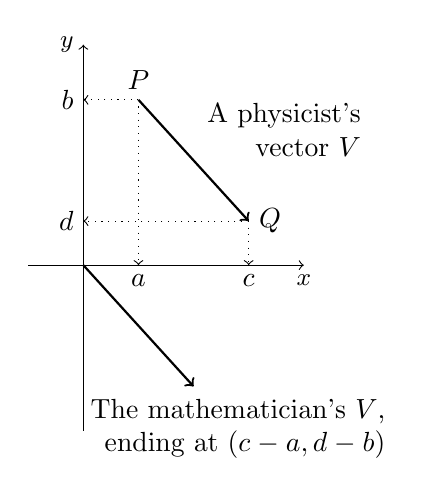
\begin{tikzpicture}[scale=1.4]
\draw[->] (-.5,0) -- (2,0) node[below] {\small $x$};
\draw[->] (0,-1.5) -- (0,2) node[left] {\small $y$};
\draw[->,thick] (1/2,3/2) node[above] {$P$} -- (3/2,2/5) node[right] {$Q$};
\node [text width=2cm,align=right,above right] at (1,18/20) {A physicist's vector $V$};
\draw[dotted,->] (1/2,3/2) -- (1/2,0) node[below] {$a$};
\draw[dotted,->] (1/2,3/2) -- (0,3/2) node[left] {$b$};
\draw[dotted,->] (3/2,2/5) -- (3/2,0) node[below] {$c$};
\draw[dotted,->] (3/2,2/5) -- (0,2/5) node[left] {$d$};
\draw[->,thick] (0,0) -- (1,-11/10);
\node [text width=3.75cm,align=right,below] at (7/5,-9/8) {The mathematician's $V$,\\ ending at $(c-a,d-b)$};
\end{tikzpicture}
\caption{The physicist's vector vs. the mathematician's vector.}
\end{figure}

But it pays to keep in mind that the physicists conception of the vector $V$ with coordinates $c-a$ and $d-b$ could be one of many different arrows, while the mathematician's vector $V$ is the arrow from the point $O = (0,0)$ to the point $(c-a, d-b)$.

Now we have circled back around to a muddle. If a mathematician's vector is always based at $O$, we only need to specify where the head of the vector is\dots which is just a point. So, how is a vector supposed to be different from a point, again? 

This confusion of three different, shifting, partially-overlapping interpretations causes some trouble to the new learner. Professionals tend to pass back and forth between these and use them flexibly to get results. Once you have gotten used to the ideas, you will, too. You should watch out for these instances where the words point and vector get interchanged. If they cause you trouble, remember that we have three different things, which are closely related.

For now, the simplest way to handle things is like this:
\begin{itemize}
\item A point is a location in the plane, and represented by coordinates in the form of an ordered pair of numbers $(a,b)$.
\item Ignore the physicist's version of the word vector as much as possible.
\item A vector is an arrow based at the origin, which can be specified by the coordinates of its head. To keep this separate from the idea of a point, we will write it differently, with the numbers stacked vertically like this: $\left(\begin{smallmatrix} a \\ b \end{smallmatrix}\right)$.
\end{itemize}
With this in mind, we make our first official definition.

\begin{definition} A $2$-vector is a vertical stack of $2$ real numbers, like so:
\[
v = \begin{pmatrix} a \\ b \end{pmatrix}.
\]
The collection of all such $2$-vectors is called \emph{the plane}, and written with this notation: $\R^2$.
\end{definition}

The notation $\R^2$ is often read ``arr-two,'' and many people use that language interchangeably with ``the plane.''

\section*{Vector Algebra}

Let's return to that glimpse of subtraction we saw in Figure \ref{fig:phys-vec-coords}.
We saw there that for points $P = (a,b)$ and $Q = (c,d)$, the vector $V$ from $P$ to $Q$ has coordinates $c-a$ and $d-b$. 
This looks almost like we subtracted the points to get $Q-P = V$. 
Can we use that? 
The weird part is that it mixes up points and vectors. 
So, we will just change viewpoints, and instead think of $P$ and $Q$ as (mathematician's) vectors:
\[
P = \begin{pmatrix} a \\ b \end{pmatrix}, \quad Q = \begin{pmatrix} c \\ d \end{pmatrix}
\]
If we put these together on the plane with the physicist's vector $V$ from $P$ to $Q$ and the mathematician's $V$ we see a wonderful triangle, and an extra vector.
\begin{figure}[h]
\centering
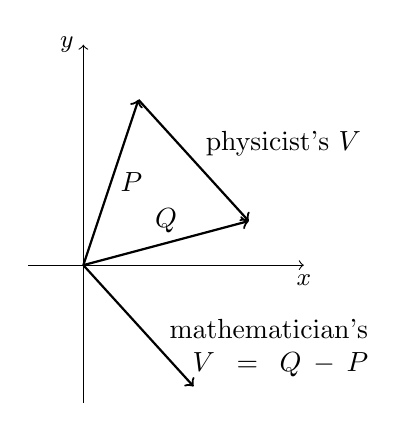
\begin{tikzpicture}[scale=1.4]
\draw[->] (-.5,0) -- (2,0) node[below] {\small $x$};
\draw[->] (0,-1.25) -- (0,2) node[left] {\small $y$};
\draw[->,thick] (1/2,3/2) -- (3/2,2/5);
\node [text width=2cm,align=right,above right] at (1,18/20) {physicist's $V$};
\draw[->,thick] (0,0) -- (1,-11/10);
\node [text width=3.5cm,align=right] at (4/3,-3/4) {mathematician's $V= Q-P$};
\draw[->,thick] (0,0) -- (1/2,3/2);
\node[right] at (1/4,3/4) {$P$};
\draw[->,thick] (0,0) -- (3/2,2/5);
\node[above] at (3/4,1/5) {$Q$};
\end{tikzpicture}
\caption{Subtraction of vectors}
\label{fig:subtract-vec}
\end{figure}
So we see a way to talk about subtracting vectors: Given two vectors $P$ and $Q$ as above, their
\emph{difference} is the vector
\[
V = Q-P = \begin{pmatrix} c \\ d \end{pmatrix} - \begin{pmatrix} a \\ b \end{pmatrix} = \begin{pmatrix} c-a \\ d-b \end{pmatrix}.
\]
Geometrically, we draw the arrow from $P$ to $Q$ and then translate it down so that its tail is at the origin $O=(0,0)$. Of course, the order of $P$ and $Q$ in this operation matters. If we switch them, we get an arrow pointing in the opposite direction.

If we can subtract vectors, surely we can add vectors. How would that work? Algebraically, if $V=Q-P$, then we expect $Q = V+P$ by rearranging. 
That would mean
\[
Q = \begin{pmatrix} c \\ d \end{pmatrix} = V + P = \begin{pmatrix} c-a \\ d-b \end{pmatrix} + \begin{pmatrix} a \\ b \end{pmatrix},
\]
which all fits. It looks like addition should be defined coordinate-by-coordinate.

\begin{definition}[Addition of Vectors]
Let $P = \left(\begin{smallmatrix} a\\ b\end{smallmatrix}\right)$ and $Q= \left(\begin{smallmatrix} c\\ d\end{smallmatrix}\right)$ be two vectors in $\R^2$. Their sum is the vector
\[
P+Q = \begin{pmatrix} a+c \\ b+d\end{pmatrix}.
\]
\end{definition}

\begin{theorem}
Addition of vectors satisfies the same rules as addition of real numbers:
\begin{compactitem}
\item when adding more than two vectors, it doesn't matter which operations you do first:
$(P+Q)+R = P + (Q+R)$;
\item one can add in either order $P+Q = Q+P$;
\item the origin $O$ is a ``zero'' since $P+O = O+P = P$;
\item for each vector $P$, there is an opposite vector $-P$ so that $P + (-P) = O$.
\end{compactitem}
\end{theorem}

Remember that you are supposed to read actively. 
You can draw all of these pictures and try out all of these things with specific examples that you invent.
You should check these by making examples and working out the details.
Can you also draw the pictures which go with your examples?

But what about subtracting geometrically? In Figure \ref{fig:subtract-vec}, I have a strong desire to complete the figure by joining the loose end of $V$ to the rest of the figure. If we draw the arrow from the head of $V$ to the head of $Q$, we get this:
\begin{figure}[h!]
\centering
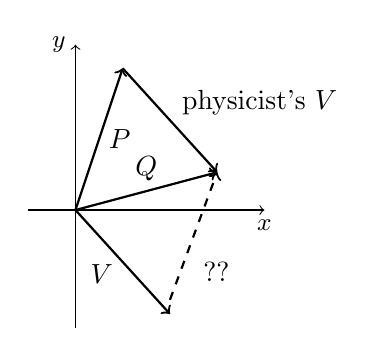
\begin{tikzpicture}[scale=1.2]
\draw[->] (-.5,0) -- (2,0) node[below] {\small $x$};
\draw[->] (0,-1.25) -- (0,1.75) node[left] {\small $y$};
\draw[->,thick] (1/2,3/2) -- (3/2,2/5);
\node [text width=2cm,align=right,above right] at (1,18/20) {physicist's $V$};
\draw[->,thick] (0,0) -- (1,-11/10);
\node [below left] at (1/2,-19/40) {$V$};
\draw[->,thick] (0,0) -- (1/2,3/2);
\node[right] at (1/4,3/4) {$P$};
\draw[->,thick] (0,0) -- (3/2,2/5);
\node[above] at (3/4,1/5) {$Q$};
\draw[->,dashed,thick] (1,-19/20) -- (3/2,2/5);
\node[right] at (5/4,-13/20) {??};
\end{tikzpicture}
\caption{Subtraction of vectors}
\label{fig:add-vec}
\end{figure}

What should the label on the dashed vector in Figure \ref{fig:add-vec} be? Just as the physicist's $V$ and the 
mathematician's $V$ are parallel, this new vector is parallel to the mathematician's vector $P$. 
So the dashed vector must be a physicist's version of $P$. Then we see $Q= V+P$.

Now we know how to add geometrically: to add two vectors $A$ and $B$, translate $B$ until its tail is on the head of $A$, then draw a new vector $A+B$ as the vector from the tail of $A$ to the head of this translated $B$. It just repurposes the structure of Figure \ref{fig:add-vec}.

\begin{figure}[h!]
\centering
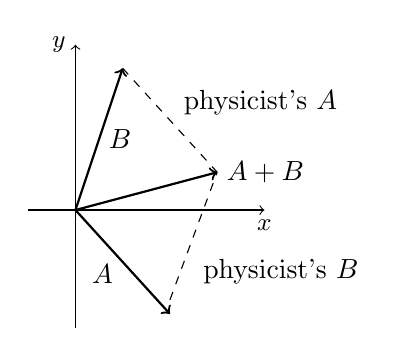
\begin{tikzpicture}[scale=1.2]
\draw[->] (-.5,0) -- (2,0) node[below] {\small $x$};
\draw[->] (0,-1.25) -- (0,1.75) node[left] {\small $y$};
\draw[-,dashed] (1/2,3/2) -- (3/2,2/5);
\node [text width=2cm,align=right,above right] at (1,18/20) {physicist's $A$};
\draw[->,thick] (0,0) -- (1,-11/10);
\node [below left] at (1/2,-19/40) {$A$};
\draw[->,thick] (0,0) -- (1/2,3/2);
\node[right] at (1/4,3/4) {$B$};
\draw[->,thick] (0,0) -- (3/2,2/5);
%\node[above] at (3/4,1/5) {$A+B$};
\draw[-,dashed] (1,-19/20) -- (3/2,2/5) node[right] {$A+B$};
\node[right] at (5/4,-13/20) {physicist's $B$};
\end{tikzpicture}
\caption{Geometric Addition of Vectors}
\label{fig:geom-add-vec}
\end{figure}

This is sometimes called the \emph{parallelogram rule} for addition of vectors.

There is another useful operation on vectors called \emph{scalar multiplication}. 
The terminology comes from physics (again) where a \emph{scalar} quantity is just a number, and not a vector.
So ``scalar multiplication'' means to multiply a vector by a scalar.


\begin{definition}[Scalar Multiplication for vectors]
Let $P = \left( \begin{smallmatrix} a \\ b \end{smallmatrix}\right)$ be a vector in $\R^2$, and let $\lambda$ be a real number. Then the scalar multiple $\lambda P$ is defined to be
\[
\lambda P = \begin{pmatrix} \lambda a \\ \lambda b \end{pmatrix}
\]
\end{definition}

If you have never seen the symbol $\lambda$ before, it is an old Greek letter pronounced ``lamb-duh.'' It is traditional to use it in linear algebra in lots of places. Welcome to the $\lambda$-club. Oh, there are others, too, like $\mu$, which is pronounced ``mew.''

Again, this operation has some important similarities to the familiar multiplication of numbers, but because it combines a scalar (a number) with a vector (not a number, exactly) to produce another vector (again, not a number) things are a little different.

\begin{theorem}
Suppose that $P$ and $Q$ are vectors, and $\lambda$ and $\mu$ are numbers. Scalar multiplication has the following properties:
\begin{compactitem}
\item Scalar multiplication distributes over vector addition:\\ $\lambda(P+Q) = \lambda P + \lambda Q$;
\item Scalar multiplication distributes over scalar addition:\\ $(\lambda + \mu)P = \lambda P + \mu P$;
\item Scalar multiplication and regular multiplication can be done in either order: $\lambda(\mu P) = (\lambda\mu) P$;
\item if $\lambda = 0$, then $\lambda P = 0 P = O$ is the zero vector $O$.
\item if $n$ is a counting number, then $nP$ is the same thing as adding together $n$ copies of $P$. In particular, $1P = P$.
\end{compactitem}
\end{theorem}

This Theorem, like the last one, just says that a bunch of natural things you expect to happen really do happen. When you study \textbf{Modern Algebra}, making lists of these kinds of properties will be really useful. So far, we have collected up the properties that describe a \emph{vector space}.


What is the geometry of scalar multiplication? 
It corresponds to stretching (or shrinking) a vector, without changing its direction.
Let $lambda$ be a non-zero number. Since 
\[
\lambda P = \lambda \begin{pmatrix} a \\ b \end{pmatrix} = \begin{pmatrix} \lambda a \\ \lambda b\end{pmatrix},
\]
we see that the ratio of the two coordinates of a vector doesn't change under scalar multiplication. This means that $P$ and $\lambda P$ point in the same direction.
One can see this be considering similar triangles with sides parallel to the $x$-axis, the $y$-axis, and $P$.

\begin{figure}[h!]
\centering
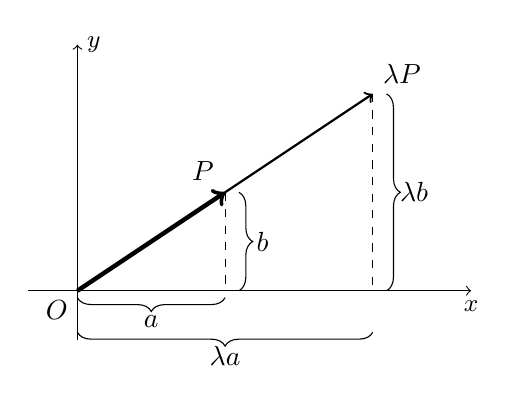
\begin{tikzpicture}[scale=1.25]
\draw[->] (-.5,0) -- (4,0) node[below] {\small $x$};
\draw[->] (0,-.5) -- (0,2.5) node[right] {\small $y$};
\node[below left] at (0,0) {$O$};
\draw[->,thick] (0,0) -- (3,2) node[above right] {$\lambda P$};
\draw[->,ultra thick] (0,0) -- (1.5,1) node[above left] {$P$};
\draw[dashed] (1.5,1) -- (1.5,0);
\draw[dashed] (3,2) -- (3,0);
\draw[decorate,decoration={brace,mirror,amplitude=5pt},xshift=4pt,yshift=0pt] (3,0) -- (3,2) node[midway,xshift=.35cm] {$\lambda b$};
\draw[decorate,decoration={brace,mirror,amplitude=5pt},xshift=4pt,yshift=0pt] (1.5,0) -- (1.5,1) node[midway,xshift=.3cm] {$b$};
\draw[decorate,decoration={brace,mirror,amplitude=5pt},xshift=0pt,yshift=-2pt] (0,0) -- (1.5,0) node[midway,yshift=-.3cm] {$a$};
\draw[decorate,decoration={brace,mirror,amplitude=5pt},xshift=0pt,yshift=-12pt] (0,0) -- (3,0) node[midway,yshift=-.3cm] {$\lambda a$};
\end{tikzpicture}
\caption{Similar triangles and scalar multiplication, $\lambda >1$}
\label{fig:sim-tri}
\end{figure}

The triangles $OXP$ and $O(\lambda X)(\lambda P)$ are similar: their corresponding horizontal and vertical sides are parallel, and those pairs of sides have a common ratio. 
We learn that $P$ and $\lambda P$ lie in the same line.

Now we are getting somewhere! We want to understand lines in the plane, and we have just discovered how scalar multiplication relates to lines which pass through the origin, $O$.

By the way, this picture helps explain the terminology. The vector $\lambda P$ is a rescaled version of $P$. A \emph{scalar} is a thing which \emph{scales} vectors.

\section*{Lines as Parametric Objects}

We see that for a non-zero vector $P$, and a non-zero number $\lambda$, the vectors $P$ and $\lambda P$ lie on the same line through the origin, $O$. But this doesn't depend on which number $\lambda$ we choose. So if we vary $\lambda$, we will get lots of different points on that line.
The picture looks something like this one:
\begin{figure}[h!]
\centering
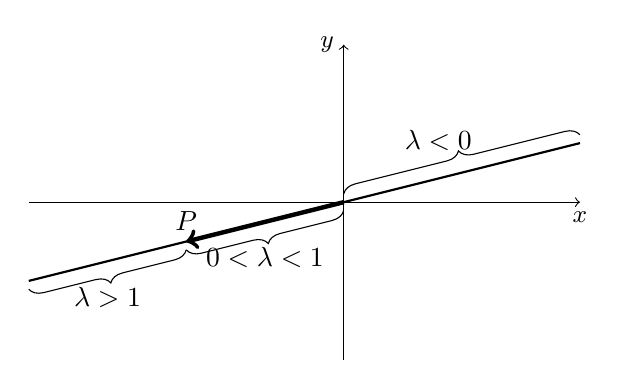
\begin{tikzpicture}
\draw[->] (-4,0) -- (3,0) node[below] {\small $x$};
\draw[->] (0,-2) -- (0,2) node[left] {\small $y$};
\draw[thick] (-4,-1) -- (3,3/4);
\draw[->,ultra thick] (0,0) -- (-2,-1/2) node[above] {$P$};
\draw[decorate,decoration={brace,amplitude=5pt,mirror},xshift=0pt,yshift=-3pt] (-4,-1) -- (-2,-1/2) node[midway,xshift=0cm,yshift=-.35cm] {$\lambda > 1$};
\draw[decorate,decoration={brace,amplitude=5pt,mirror},xshift=0pt,yshift=-3pt] (-2,-1/2) -- (0,0) node[midway,xshift=0cm,yshift=-.35cm] {$0< \lambda <1$};
\draw[decorate,decoration={brace,amplitude=5pt},xshift=0pt,yshift=3pt] (0,0) -- (3,3/4) node[midway,xshift=-.3cm,yshift=.3cm] {$\lambda <0$};
\end{tikzpicture}
\caption{The points on a line: $\lambda P$ for different $\lambda$}
\label{fig:line-scalar}
\end{figure}

This leads us to what is called a \emph{parametric description} of the line.
We think of some variable, say $t$, as a parameter.
(I chose $t$ here so that we think of it as ``time.'')
As we change the value of $t$, the vectors $tP$ trace out the line which goes through the origin and the point which is the head of the vector $P$.

\begin{theorem}[parametric lines through the origin] \label{thm:param-line-origin}
Suppose that $P=(a,b)$ is some point in the plane. The the line which passes through the origin $O$ and the point $P$ consists of the heads of all the vectors 
\[
t \begin{pmatrix} a \\ b \end{pmatrix},
\]
where $t$ varies over all real numbers. That is, this line is the set of the heads of all scalar multiples of the vector corresponding to $P$.
\end{theorem}

This, is fantastic. We can use simple vector algebra to describe any line through the origin. 
What about lines that are not through the origin? 
Suppose we just have two random points $P$ and $Q$, neither of which is the origin, and we want to describe the line $\ell$ through $P$ and $Q$?

Again, let's think of the points on this line $\ell$ as the heads of mathematics-style vectors. 
If we put in the vectors $p$ and $q$ which correspond to the points $P$ and $Q$, we get a good picture like this one.

\begin{figure}[h!]
\centering
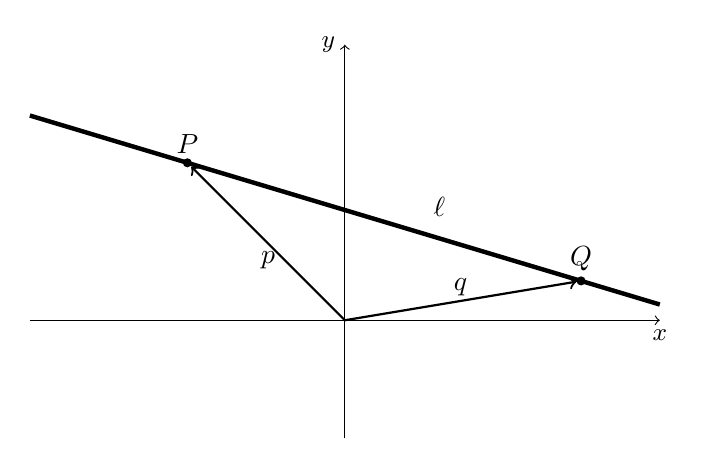
\begin{tikzpicture}[scale=1]
\draw[->] (-4,0) -- (4,0) node[below] {\small $x$};
\draw[->] (0,-1.5) -- (0,3.5) node[left] {\small $y$};
\draw[fill] (-2,2) circle [radius=.05]; 
\node[above] at (-2,2) {$P$};
\draw[fill] (3,.5) circle [radius=.05];
\node[above] at (3,.5) {$Q$};
\draw[ultra thick] (-4,2.6) -- (4,.2);
\node[above] at (1.2,1.2) {$\ell$};
\draw[->,thick] (0,0) -- (-1.95,1.95) node[midway,yshift=-6pt] {$p$};
\draw[->,thick] (0,0) -- (2.94,.49) node[midway,yshift=5pt] {$q$};
\end{tikzpicture}
\caption{Working toward a parametric line, part 1}
\label{fig:param-line1}
\end{figure}

Each point in Figure \ref{fig:param-line1} is the head of a vector from the origin to that point. 
In particular, the point $P$ is the head of the vector $p$. 
So if we add $-p$ to every single one of these, we will move the whole line $\ell$ in the direction and with the same distance as $-p$.
That will make a new line, $\ell'$, and the point which comes from $P$ will land on the origin.


\begin{figure}[h!]
\centering
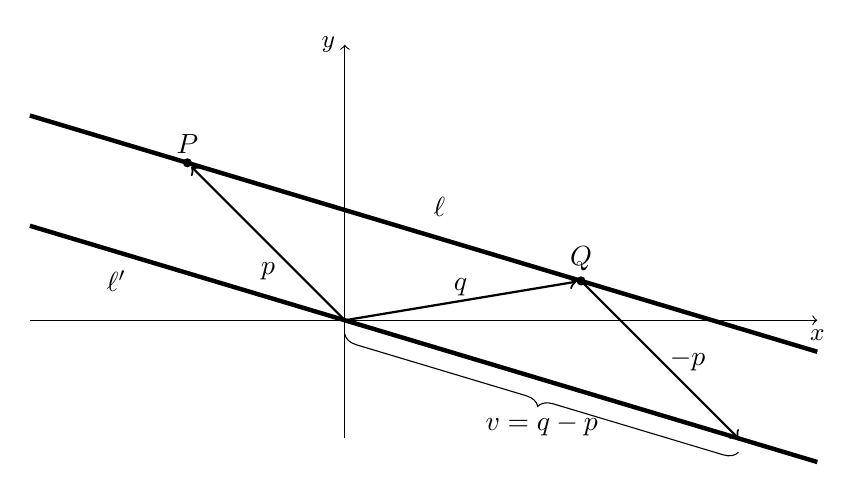
\begin{tikzpicture}[scale=1]
\draw[->] (-4,0) -- (6,0) node[below] {\small $x$};
\draw[->] (0,-1.5) -- (0,3.5) node[left] {\small $y$};
\draw[fill] (-2,2) circle [radius=.05]; 
\node[above] at (-2,2) {$P$};
\draw[fill] (3,.5) circle [radius=.05];
\node[above] at (3,.5) {$Q$};
\draw[ultra thick] (-4,2.6) -- (6,-.4);
\node[above] at (1.2,1.2) {$\ell$};
\draw[->,thick] (0,0) -- (-1.95,1.95) node[midway,yshift=-10pt] {$p$};
\draw[->,thick] (0,0) -- (2.94,.49) node[midway,yshift=5pt] {$q$};
\draw[ultra thick] (-4,1.2) -- (6,-1.8);
\node at (-2.9,.5) {$\ell'$};
\draw[->,thick] (3,.5) -- (5,-1.5) node[midway,xshift=10pt] {$-p$};
\draw[decorate,decoration={brace,amplitude=5pt,mirror},xshift=0pt,yshift=-5pt] (0,0) -- (5,-1.5) node[midway,yshift=-.41cm] {$v = q-p$};
\end{tikzpicture}
\caption{Working toward a parametric line, part 2}
\label{fig:param-line2}
\end{figure}

Since $q$ is one of the vectors with its head on the original line, the vector $q-p$ will have its head on the new line, too.
But $q-p$ has its tail at the origin! 
So, our new line passes through the origin and the head of the vector $q-p$, and we are in a situation to apply Theorem \ref{thm:param-line-origin}.


By Theorem \ref{thm:param-line-origin}, the line $\ell'$ is described as all of the points which are heads of vectors of the form
$t (q-p)$, where $t$ is a parameter which is allowed to vary over all real numbers.
But we get from $\ell'$ back to $\ell$ by simply adding the vector $p$ back in. 
So, our original line $\ell$, which goes through the heads of vectors $p$ and $q$, is described as the set heads of the vectors 
\[
p + t (q-p),
\] 
where $t$ is a parameter which is allowed to vary over all real numbers.
Now, let's sum up what we have learned.

\begin{theorem}[parametric line]\label{thm:param-line}
Let $P = (a,b)$ and $Q = (c,d)$ be two points in the plane. The line which passes through these two points can be described as the heads of all vectors of the form
\[
\begin{pmatrix} a \\ b \end{pmatrix} + t \begin{pmatrix} c-a \\ d-b\end{pmatrix},
\]
where $t$ is a parameter which is allowed to vary over all real numbers.
\end{theorem}

Note that this theorem actually includes the previous one as a special case. 
If one of our points happens to be the origin, we simply use $P=O$, which corresponds to the zero vector, and this description collapses back into the one we found earlier.
In either case, the vector $v= q-p$ is called a \emph{direction vector} for the line.


As a bit of a palate cleanser, let's answer this: Suppose you are given a line described as in the last theorem. How would you sketch it in the plane? The simplest method is to choose two different values of $t$, use them to generate to points on the line, plot those points, and trace the line through them. Which values of $t$ should you choose? It is often convenient to use $t=0$ and $t=1$.



\section*{Lengths and Angles in the plane}
\begin{compactitem}
\item lengths, angles, and the dot product in R2
\item normal vector to a line in R2
\item duality
\end{compactitem}


\section*{Lines and Equations}
\begin{compactitem}
\item equation of a line, three methods: elimination, from two pts via similar triangles, from geometry of dot product
\item families of parallel lines
\item sketching a line from an equation
\end{compactitem}

\section*{Conclusion: The Big Theorem}


\end{document}